 \chapter{Analytic approximations and calculations}
 
\section{Rate equations for leptogenesis}
In order to qualitatively describe leptogenesis one has to consider rate equations for the lepton number and B-L number densities. In a static universe without lepton number violating processes the rate equation would trivially be
\begin{equation}
	\frac{d}{dt}n=0.
	\label{eq:rate_static_nointeraction}
\end{equation}
If one now condsiders a universe expanding with the rate H the rate equation above changes to
\begin{equation}
\left(\frac{d}{dt}+3H\right)n=0.
\label{eq:rate_expanding_nointeraction}
\end{equation}
Finally including lepton number violating processes the rate equation one obtains for the neutrino number density is
\begin{equation}
\left(\frac{d}{dt}+3H\right)n_N=-\Gamma_N\left(n_N-n_N^{eq}\right)+\Gamma_{N,B-L}n_{B-L}.
\label{eq:L_rate_expanding_interaction}
\end{equation}
Applying this reasoning to the B-L number density yields
\begin{equation}
\left(\frac{d}{dt}+3H\right)n_{B-L}=\Gamma_{B-L,N}\left(n_N-n_N^{eq}\right)-\Gamma_{B-L}n_{B-L}.
\label{eq:B-L_rate_expanding_interaction}
\end{equation}
The coefficient $\Gamma_N$ denotes how fast the neutrino density equalizes with its equilibrium density, while $\Gamma_{B-L}$ describes the washout of a net B-L number. $\Gamma_{B-L,N}$ describes how the B-L asymmetry is affected by the deviation of the neutrino density from its equilibrium value and together with $\Gamma_{N,B-L}$ these two coefficients characterize CP violating processes \cite[p. 4]{Bodeker:2013qaa}. Since both these coefficients describe CP violating processes they must depend on the CP violating parameter $\epsilon$ introduced in the section before and it was also shwon there that this parameter is small for heavy neutrino decays and because $n_{B-L}\ll\left(n_N-n_N^{eq}\right)$ the second term in equation \eqref{eq:L_rate_expanding_interaction} can be neglegted. \newline\indent
The goal now is to determine these coefficients at least at leading order and the first one will be $\Gamma_N$. To get this coefficient one has to integrate equation \eqref{eq:L_rate_expanding_interaction} over phase space, resulting in
\begin{equation}
	\left(\frac{\partial}{\partial t}-Hp\frac{\partial}{\partial p}\right)f_N=\Gamma_N\left(e^{E_N/T}-f_N\right).
	\label{eq:boltzmann}
\end{equation}
The whole calculation on how to perform the phase space integral can be found in appendix \ref{ap:phase_space}. \newline\indent
One might now notice that equation \eqref{eq:boltzmann} differs from equation 4 in \cite{Bodeker:2013qaa} by a factor of M$_N$/E$_N$, that origins in a different normaliziation of the phase space. However, since we operate in a non-relativistic regime E\textsubscript{N} $\approx$ M\textsubscript{N}, therefore this factor is $\sim$ 1 and negligible. Using this argumentation one can also see that $\Gamma_N=\Gamma_0$ with $\Gamma_0$ the total decay rate of the heavy neutrinos, which is governed by the Yukawa interaction term \eqref{eq:Yukterm}. It has to be mentioned that for the equilibrium distribution the Boltzmann statistic with neglegted chemical potential was used since the energy of a neutrino E\textsubscript{N} $\approx$ M\textsubscript{N} $\gg$ T during the phase where the decay happen outside equilibrium and therefore quantum mechanical effects play an insignificant role and can be neglected. Going back to the decay rate, that can be calculated as done in appendix \ref{ap:tree_level_decay}, one gets
\begin{equation}
\Gamma_N=\Gamma_0=\frac{|h_{11}|^2M_N}{8\pi}.
\label{eq:Gamma_N}
\end{equation}
As explained above $\Gamma_{B-L,N}$ connects the B-L asymmetry with the deviation of n\textsubscript{N} from its equilibrium value and because the only processes able to produce a B-L asymmetry  are the decays of the heavy neutrino and therefore $\Gamma_{B-L,N}$ is directly connected to its decay rate. On the other hand though, any B-L asymmetry can only arise through CP violation, meaning the neutrino has to decay into leptons and anti-leptons at different rates. The parameter describing this difference is $\epsilon$, as it is given in \eqref{eq:CP_violation}. Putting all this together results in 
\begin{equation}
	\Gamma_{B-L,N}=\epsilon\Gamma_0.
	\label{eq:Gamma_B-L,N}
\end{equation}
The last coefficient left to determine is $\Gamma_{B-L}$. This one however refers to the washout of the B-L asymmetry hence it arises from the inverse decay $\ell\phi\rightarrow$ N. It can be calculated using the quatum field theoretical means for obtaining decay rates and taking into account that particle distributions and neutrino momenta have to be considered because of non-zero temperatures.
\begin{equation}
\Gamma_{B-L}n_{B-L}=\int\prod_{a=N,\ell,\phi}\frac{d^3p_a}{2E_a(2\pi)^3}(2\pi)^4\delta(p_\ell+p_\phi-p_N)(	f_\ell f_\phi-f_{\bar{\ell}}f_{\bar{\phi}})\sum|M_0|^2,
\label{eq:Gamma_B-L}
\end{equation}
where $\sum|M_0|^2=16\pi M_N\Gamma_0$ describes the tree level matrix element for exactly this inverse decay summed over all spins of N and isospin components of $\ell$. In order to evaluate this integral properly one has to first describe the term $(	f_lf_\phi-f_{\bar{l}}f_{\bar{\phi}})$ more precisely. Since we operate at rather high temperatures one can use Boltzmann statistics for lepton and Higgs regardless and expanding in the chemical potentials up to first order yields.
\begin{equation}
	f_\ell f_\phi-f_{\bar{\ell}}f_{\bar{\phi}}\simeq 2e^{-\frac{E_N}{T}}\frac{\mu_l+\mu_\phi}{T}.
	\label{eq:distri_diff}
\end{equation}
As mentioned in \cite[p. 7]{Bodeker:2013qaa} the chemical potentials are proportional to the B-L number density and by using the coefficients $c_l$ and $c_\phi$ in order to avoid introducing the exact temperature dependant relations one can also connect n$_{B-L}$ to the lepton and Higgs asymmetries through \cite[p. 7]{Bodeker:2013qaa}
\begin{align}
	n_\ell-n_{\bar{\ell}}=-c_\ell n_{B-L},
	\label{eq:l-lbar} \\
	n_\phi-n_{\bar{\phi}}=-c_\phi n_{B-L},
	\label{eq:phi-phibar}
\end{align}
Different values for $c_l$ and $c_\phi$ then correspond to different temperature ranges that are given in table \ref{tab:temperatur}\cite[Table 1]{Bodeker:2013qaa}.

	\begin{table}[H]
	\centering
	\begin{tabular}{c|c||c}
	T (GeV)& $c_l$ & $c_\phi$\\
	\hline
	$\ll10^{13}$&1&2/3\\
	$\sim10^{13}$&1&14/23\\
	$10^{12}-10^{13}$&3/4&1/2\\
	$10^{12}-10^{13}$&78/115&56/115\\
	$10^{12}-10^{13}$&344/537&52/179\\
	
	\end{tabular}
	\caption{Values of $c_l$ and $c_\phi$ for different temperature ranges}
	\label{tab:temperatur}
	\end{table}

Now by expanding the number distribution for leptons and Higgs and their respective anti particles in the chemical potentials up to first order one can finally put the chemical potential and n$_{B-L}$ in relation to each other. It is important to note that one has to use the Fermi-Dirac- and Bose-Einstein distribution for leptons and Higgses respectively. The reason for this is that these two particle species are in equilibrium at the temperature T. Because of this and the fact that they are relativistic particles, their kinetic energy and therefore momenta are of order T and quantum effects cannot be neglected. On the other hand it is possible to use Boltzmann statistics for leptons and Higgs bosons above since particles taking part in the production of a heavy neutrinos having energies or momenta of order M\textsubscript{N}/2 $\gg T$ and quantum effects can safely be neglected in this case. Finally using quantum statistics results in
\begin{align}
\mu_\ell=\frac{3c_l}{T^2}n_{B-L},
\label{eq:chempot_l}
\\
\mu_\phi=\frac{3c_l}{2T^2}n_{B-L}.
\label{eq:chempot_phi}
\end{align}
Using all these results and putting them into relation \eqref{eq:Gamma_B-L} one gets the following result for the washout rate $\Gamma$\textsubscript{B-L}
\begin{equation}
	\Gamma\textsubscript{B-L}=\frac{3}{\pi^2}\:\left(c_\ell+\frac{c_\phi}{2}\right)z^2K_1(z)\Gamma_0,
	\label{eq:Gamma_B-l_result}
\end{equation}
with K\textsubscript{1}(z) the modified Bessel function of the second kind and 
\begin{equation}
	z\equiv\frac{M_N}{T}.
\end{equation}
This can be seen as a dimensionless measure for time, since the temperature of the universe decreases over time and therefore z increases. 
The exact derivation of these results can be looked up in appendix \ref{ap:Gamma_B-L}. \newline\indent
Using the relations given in \eqref{eq:rate_g_hubble} and \eqref{eq:rate_s_hubble} it is usefull to define the so called wash out factor K as follows
\begin{equation}
	K\equiv\left.\frac{\Gamma_0}{H}\right|_{T=M\textsubscript{N}}.
	\label{eq:washout}
\end{equation}
Using this and equation 3 of \cite{Buchmuller:2004nz}
\begin{equation}
	H(z)=\left.H\right|\textsubscript{T=M\textsubscript{N}}\cdot \frac{1}{z^2},
	\label{eq:H_von_z}
\end{equation}
one can now compare the rates calculated above to the Hubble constant H.\newline\indent
For T $\lesssim$ M\textsubscript{N} one can approximate $\Gamma\textsubscript{N}$ as $\Gamma_0$ resulting in 
\begin{equation}
	\frac{\Gamma_\textsubscript{N}}{H}\simeq\frac{\Gamma_0}{\frac{1}{z^2}\left.H\right|\textsubscript{T=M\textsubscript{N}}}=z^2K.
	\label{eq:Gamma_N_H}
\end{equation}
Since z increases with time, equation \eqref{eq:Gamma_N_H} clearly shows that the rate with which the neutrino number density approaches its equilibrium value gets greater than the expansion of the universe and therefore the deviation from equilibrium vanishes over time. \newline\indent
Looking at \eqref{eq:Gamma_B-l_result} one can easily see that for T $\sim$ M\textsubscript{N}, or z $\approx$ 1, $\Gamma\textsubscript{B-L}$ is of the same order as $\Gamma\textsubscript{N}$, since K$_1$(1)=$\mathcal{O}$(1). On the other hand however, for really low temperatures, meaning T $\ll$ M\textsubscript{N} or z very big, one can see the quantitative behaviour of $\Gamma\textsubscript{B-L}$ by using the asymptotic expansion of the modified Bessel function given by
\begin{equation*}
	K\textsubscript{n}(z)\sim\sqrt{\frac{\pi}{2z}}e^{-z}\sum_{k=0}^{\infty}\frac{a\textsubscript{k}(n)}{z^k},
\end{equation*}
with $a$\textsubscript{k}(n) some coefficients that are not of any interest for this matter. Now using this and dropping all but the first term of the sum above, which is justified because z is large, one gets
\begin{equation}
	\frac{\Gamma\textsubscript{B-L}}{H}\sim\sqrt{\frac{1}{z}}e^{-z}z^2\frac{\Gamma_0}{\frac{1}{z^2}\left.H\right|\textsubscript{T=M\textsubscript{N}}}=z^\frac{7}{2}e^{-z}K.
	\label{eq:Gamma_B-L_H}
\end{equation}
So because $\Gamma\textsubscript{N}$ increases with z for z $\approx$ 1 so does $\Gamma\textsubscript{B-L}$. However, as equation \eqref{eq:Gamma_B-L_H} suggests, $\Gamma\textsubscript{B-L}$ gets more and more suppressed by the exponential factor for increasing z and therefore has to have some maximum. Additionally for sufficiently low temperatures, like the extremely low 2.7K of the present universe, the washouth rate $\Gamma\textsubscript{B-L}$ is effectively zero and any symmetry produced in earlier times is frozen out. 
All this can be seen in figure \ref{fig:rates} where the previously calculated ratios are plotted against z and are normalized to the washout factor K.
\begin{figure}[H]
	\centering
	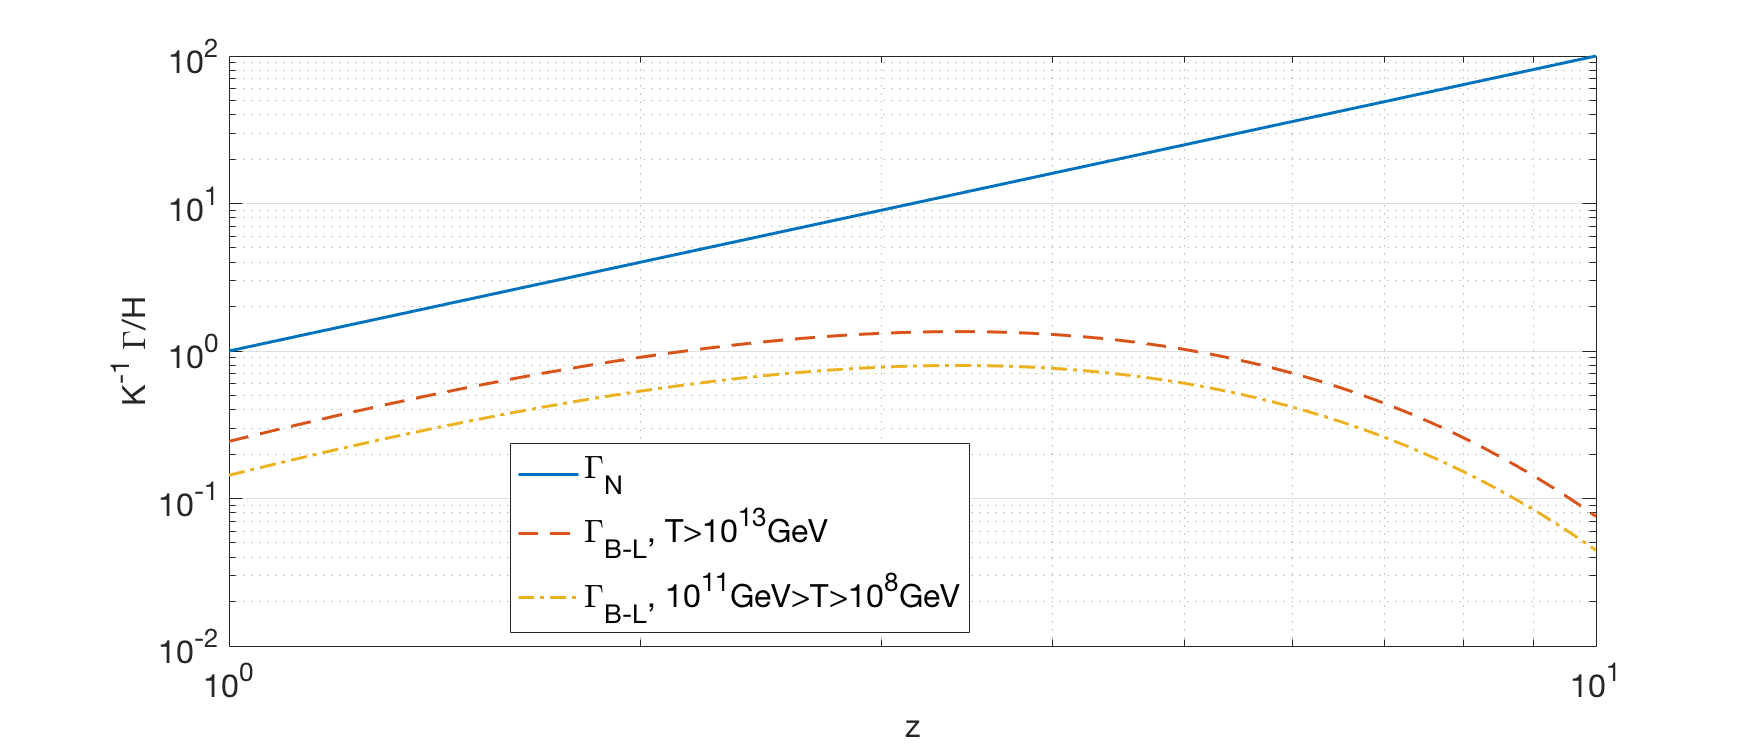
\includegraphics[width=0.8\linewidth]{Images/rates}
	\caption{The ratios $\Gamma\textsubscript{N}$/H and $\Gamma\textsubscript{B-L}$/H plotted against H}
	\label{fig:rates}
\end{figure}
\section{Relativistic corections}
Although this thesis focuses on a non-relativistic scenario for leptogenesis it might be interesting to see how much relativistic corrections influence the previous results. For this matter one has to reintroduce the factor M\textsubscript{N}/E\textsubscript{N} seen in equation 4 of \cite{Bodeker:2013qaa}, that was dropped in equation \eqref{eq:boltzmann} since it simplifies to 1 in the non-relativistic limit, so this equation reads
\begin{equation}
	\left(\frac{\partial}{\partial t}-Hp\frac{\partial}{\partial p}\right)f_N=\frac{M_N\Gamma_0}{E_N}\left(e^{E_N/T}-f_N\right).
	\label{eq:boltzmann_2}
\end{equation}
Now, using the relativistic energy-momentum relation,
\begin{equation}
	E=\sqrt{M^2+p^2},
	\label{eq:rel_energy_momentum}
\end{equation}
one can expand the factor 1/E$_N$ on the right-hand side up to order p$^2$ and therefore get the next-to-leading order relativisitic corrections for the rate equation \eqref{eq:L_rate_expanding_interaction}
\begin{equation}
\left(\frac{d}{dt}+3H\right)n_N=\Gamma_N\left(n_N^{eq}-n_N\right)+\Gamma_{N,u}\left(u-u^{eq}\right),
\label{eq:L_rate_expanding_interaction_rel}
\end{equation}
with u the kinetic energy density of the heavy neutrinos divided by their mass
\begin{equation}
	u=\frac{g_N}{M_N}\int\frac{d^3p}{(2\pi)^3}\:\frac{p^2}{2M_N}f_N,
	\label{eq:energy_density}
\end{equation}
with g$_N$ the the internal degrees of freedom of the neutrinos. \newline\indent
By multiplying \eqref{eq:L_rate_expanding_interaction_rel} with p$^2$ and integrating over p one can easily get a rate equation for u, which at leading order in p, so for E$_N$=M$_N$, reads as
\begin{equation}
	\left(\frac{d}{dt}+5H\right)u=\Gamma_u\left(u^{eq}-u\right).
	\label{eq:rate_u}
\end{equation}
It is important to note that for the rates appearing above, the following relations are holding
\begin{align}
	\Gamma_{N,u}=\Gamma_{0},
	\label{eq:Gamma_N,u}
	\\
	\Gamma_{u}=\Gamma_{0}.
	\label{eq:Gamma_u}
\end{align}
Now again by expanding the factor 1/E$_N$ one gets an equivalent expansion for equation \eqref{eq:B-L_rate_expanding_interaction}. Since the B-L asymmetry density is not directly affected by any relativistic effects, only the term containing the neutrino density has to be expanded, resulting in
%\todo{Minus}
\begin{equation}
	\left(\frac{d}{dt}+3H\right)n_{B-L}=\Gamma_{B-L,N}\left(n_N-n_N^{eq}\right)-\Gamma_{B-L,u}\left(u-u^{eq}\right)+\Gamma_{B-L}n_{B-L}.
	\label{eq:B-L_rate_expanding_interaction_rel}
\end{equation}
At lowest order in relativistic corrections, similarly to \eqref{eq:Gamma_B-L,N}, one gets
\begin{equation}
	\Gamma_{B-L,u}=\epsilon\Gamma_0.
	\label{eq:Gamma_B-L,u}
\end{equation}
How exactly these corrected rate equations are obtained can be looked up in appendix \ref{ap:rel_corrections}.
\section{Radiative corrections}
Until now only the decays and inverse decays of heavy neutrinos, so 1 $\leftrightarrow$ 2 processes have been considered, but naturally there are more processes that affect the neutrino density and therefore the asymmetry n$_{B-L}$ like 2 $\leftrightarrow$ 2 scattering, 1 $\leftrightarrow$ 3 decays and virtual corrections to the already treated 1 $\leftrightarrow$ 2 decays. \newline\indent
Since the density n$_{B-L}$ does not describe actual particles but only the B-L asymmetry relativistic corrections will only affect the neutrino densities or rather the rates associated with these densities. Furthermore it can be shown that the radiative corrections to the number distribution f$_N$ to the change over time, so f$_N$/dt, for n$_N$=0 has the following form \cite{Laine:2011pq}
\begin{equation}
\left.\frac{\partial f_N}{\partial t}\right|_{f_N=0}=f^{eq}\:\Gamma_0\frac{M_N}{E_N}\left[a+\frac{p^2}{M_N^2}b+\mathcal{O}\left(\frac{p^4}{M_N^4}\right)\right],
\label{eq:df_dt}
\end{equation}
with a and b the following temperature-dependant coefficients
\begin{align}
a&=1-\frac{\lambda T^2}{M_N^2}-\left|h_t\right|^2\left[\frac{21}{2(4\pi)^2}+\frac{7\pi^2}{60}\frac{T^4}{M_N^4}\right]+\left(g_1^2+3g_2^2\right)\left[\frac{29}{8\left(4\pi\right)^4}-\frac{\pi^2}{80}\frac{T^4}{M_N^4}\right]\\
\nonumber
&+\mathcal{O}\left(g^2\frac{T^6}{M_N^6},g^3\frac{T^2}{M_N^2}\right),\\
b&=-\left[\left|h_t\right|^2\frac{7\pi^2}{45}+\left(g_1^2+3g_2^2\right)\frac{\pi^2}{60}\right]\frac{T^4}{M_N^4}+\mathcal{O}\left(g^2\frac{T^6}{M_N^6},g^3\frac{T^2}{M_N^2}\right).
\end{align}
h$_t$ here denotes the Yukawa coupling of top quarks to the Higgs field, g$_1$ and g$_2$ are the U(1) and SU(2) gauge couplings and $\lambda$ again the Higgs self-coupling. \newline\indent
Plugging equation \eqref{eq:df_dt} into \eqref{eq:B-L_rate_expanding_interaction_rel} and \eqref{eq:rate_u} one gets the radiative corrections for $\Gamma_N$, $\Gamma_u$ and $\Gamma_{Nu}$ by expandig the E$_N$ factor in \eqref{eq:df_dt} just as done for obtaining the relativistic corrections and then integrating over the momentum. The results of this procedure that can be looked up in appendix \ref{ap:rad_corrections}, are at leading order of the respective equation,
%\todo{1/2 klären}
\begin{align}
	\Gamma_N=&\Gamma_u=a\Gamma_0,\\
	\Gamma_{N,u}=&(a-2b)\Gamma_0.
\end{align}
One thing interesting to note about the coefficients a and b is the following. The term of lowest order in T in these two coefficients is proportional to T$^2$/M$_N^2$, which corresponds to $\mathcal{O}(p^4)$ because E=$p^2/M_N\sim$ T and therefore p$^2\sim$ T/M$_N$. This would imply that the relativistic corrections should be calculated up to an order of at least p$^4$, but, as will be obvious later, these corrections of order p$^2$ are already really small.
